\chapter[Resultados]{Resultados}

A partir do estudo e pesquisa realizado até o momento determinamos o que utilizar no conjunto do sistema, levantando um perfil que a equipe acredita ser a mais viável em termos de interação, custo-benefício, tempo, conhecimento técnico e outros fatores importantes para o projeto. Será desenvolvido um kit com capacidade de ser acoplado em diversas cadeiras de rodas afim de facilitar a mobilidade elétrica em cadeiras manuais. Os resultados levantados estão disposto no decorrer do capítulo.

\section{Estrutura}

Com a utilização do programa CATIA V5 3D foi estruturado o sistema eletrônico acoplado à cadeira de rodas, \ref{fig:vista_isometrica_traseira}. Visando três preceitos básicos: comodidade, acessibilidade e conforto.

\begin{figure}[!htb]
\centering
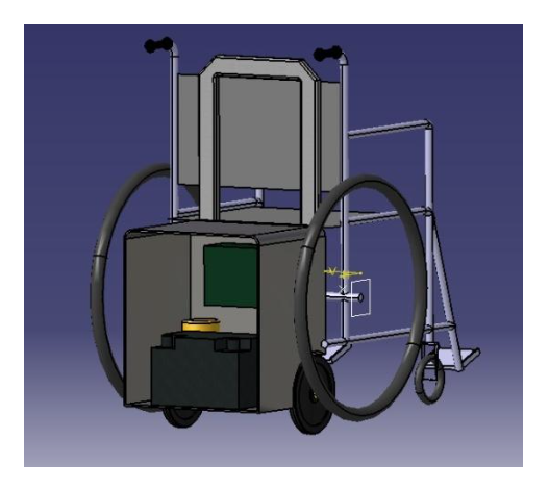
\includegraphics[keepaspectratio=true,scale=0.4]{figuras/estrutura/vista_isometrica_traseira}
\caption{Vista Isométrica Traseira}
\label{fig:vista_isometrica_traseira}
\end{figure}

O objetivo do projeto é desenvolver uma estrutura de fácil conexão e resistente. O produto proposto, ver figura \ref{fig:traseira},\ref{fig:sistema}, \ref{fig:lateral} e \ref{fig:superior},deve-se acoplar a qualquer cadeira de rodas. Foi pensado em um dispositivo no formato de uma mala para que seja de fácil conexão, uso e manuseio.

\begin{figure}[!htb]
\centering
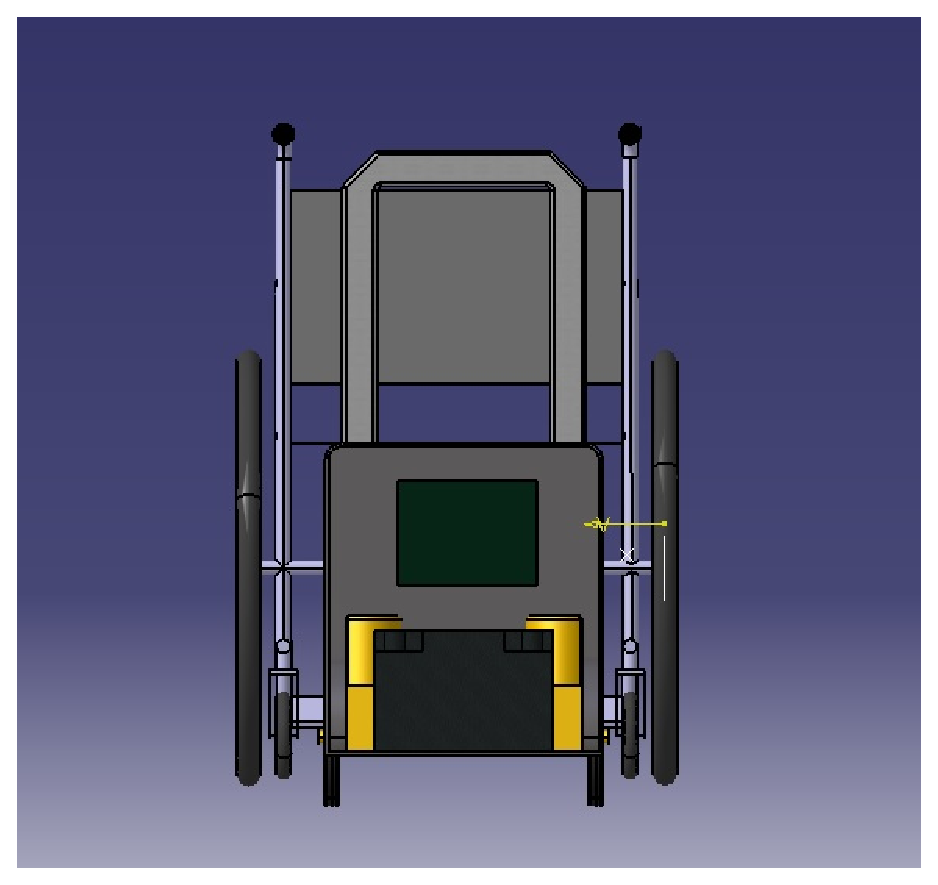
\includegraphics[keepaspectratio=true,scale=0.4]{figuras/estrutura/vista_traseira}
\caption{Vista Traseira}
\label{fig:traseira}
\end{figure}

A forma como a mala será acoplada a cadeira usa como base as hastes da mala e as hastes verticais aonde as manoplas utilizadas para empurrar manualmente a cadeira são fixadas. Tendo em vista que são rígidas e normatizadas pela NBR 9050 as hastes verticais da cadeira tem a distancia e espessura já definidas, o que facilita o desenvolvimento de um produto que possa ser usado em qualquer cadeira de rodas que esteja dentro dos padrões impostos pela norma.

\begin{figure}[!htb]
\centering
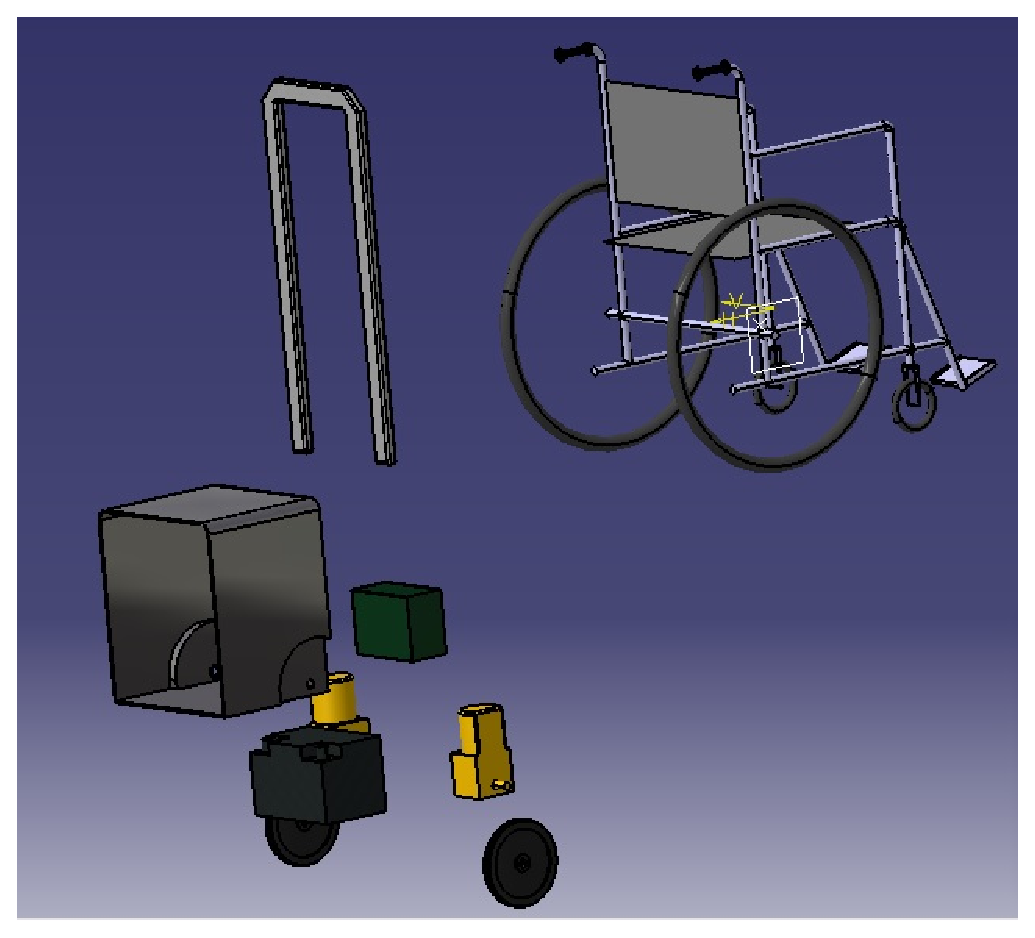
\includegraphics[keepaspectratio=true,scale=0.4]{figuras/estrutura/explode}
\caption{Visão do Sistema}
\label{fig:sistema}
\end{figure}

Cada roda possuirá um motor próprio para que seja possível rotaciona-lás em sentidos opostos, por exemplo, quando for necessário fazer manobras em que a rotação deve ocorre em torno do eixo do próprio cadeirante, movimento muito comum para manobrar uma cadeira de rodas. Assim o cadeirante se sentira confortável e não terá grandes dificuldades quando for manobrar a cadeira, já que a lógica de controle será a mesma usada quando se propulsiona manualmente a cadeira.

\begin{figure}[!htb]
\centering
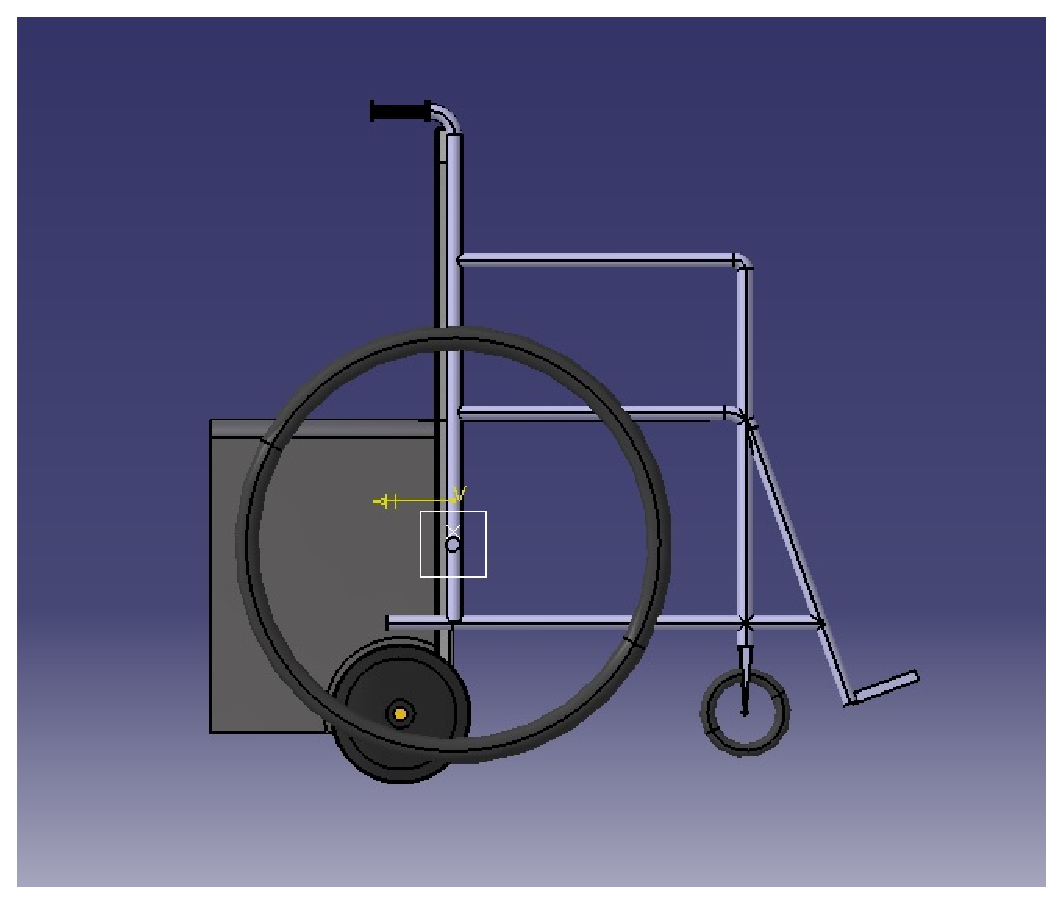
\includegraphics[keepaspectratio=true,scale=0.4]{figuras/estrutura/vista_lateral_cadeira}
\caption{Imagem Lateral}
\label{fig:lateral}
\end{figure}

Como pode se notar nas figuras, o sistema de propulsão devera empurrar a cadeira de rodas, pois assim podemos aproximar o máximo possível o eixo da roda que ira gerar o movimento ao eixo da maior roda da cadeira, o que diminui a quantidade de torque necessário para movimentar o conjunto, fazendo com que o consumo de energia diminua e possibilite o uso de um motor de menor potencia, que diminuirá o custo do produto final.

\begin{figure}[!htb]
\centering
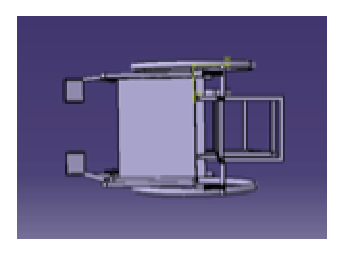
\includegraphics[keepaspectratio=true,scale=0.4]{figuras/estrutura/vista_superior}
\caption{Imagem Superior}
\label{fig:superior}
\end{figure}

\section{Power Train}
\subsection{Motor}

Será utilizado no projeto o motor de corrente contínua. A escolha foi feita pois esse tipo de motor é muito utilizado em projetos que necessitam de velocidades variáveis, eles também apresentam uma região de torque e potência constante e são simples de realizar a aceleração e a desaceleração \cite{manual_bateria_unipower}.

Especificações a serem atendidas:
\begin{itemize}
 \item Velocidade máxima de 7,44km/h;
 \item Peso máximo de 120 kg;
 \item Peso da bateria 10 kg;
 \item Peso da cadeira (valor aproximado) 20kg;
 \item Peso total estimado: 150 Kg;
 \item Considerando hipoteticamente o coeficiente de atrito ($\mu$): 0,2.
\end{itemize}


\subsection{Baterias}
A bateria de chumbo-ácido é muito utilizada hoje em dia em diferentes áreas,  como automóveis, sistemas de fornecimento de energia elétrica ininterrupta (no-breaks) e cadeiras de rodas elétricas. Desprezando-se o problema do peso e considerando as observações feitas anteriormente no capítulo \ref{cap:fundamentacao_teorica} foi a bateria escolhida para o projeto, considerando ainda o seu fácil acesso e baixo  custo.

\subsubsection{Autonomia}

Segundo a literatura, cadeiras de rodas elétricas trabalham com motores de corrente contínua entre 250 W a 300 W de potência. Para este projeto se decidiu utilizar motores de 300W. Há diversas maneiras de chegar neste valor, como por distribuição de forças, por balanço de energia, por forças em um plano inclinado, entre outras. Para este projeto fez-se uma estimativa da potência necessária através do balanço de energia.

	A energia fornecida pelo motor deve ser igual à energia cinética da cadeira. Sendo a massa máxima que a cadeira de rodas aguenta de 150 kg e considerando que cadeiras de rodas elétricas chegam até 10 km/h, tem-se:

\begin{equation}
 Em_{x} = \frac{m*V^{2}}{2} * \varepsilon
\end{equation}

        	Onde Em é a energia fornecida pelo motor, m é a massa de 150 kg e V é a velocidade em m/s. Aqui estimou-se perdas do motor de pelo menos 20\%, sendo assim,  é igual a 1,20. Assim, a energia necessária para mover a cadeira é de 694.44 J, a potência é portanto 694.44 W.

        	Ao utilizar dois motores de 300 W, a potência total entregue ao sistema seria de 600 W. Rearranjando a equação para encontrar o valor da velocidade, e atribuindo 80\% de eficiência no acoplamento das rodas com o eixo do motor, temos:

\begin{equation}
  V_{x} =  0.8 * \sqrt { \frac{600*2}{m* \varepsilon}}
\end{equation}

        	Assim, a estimativa da velocidade máxima que a cadeira deve obter será de pelo menos 7.44 km/h, que é uma velocidade razoável para este tipo de sistema. Sabe-se que a velocidade angular é dada pela divisão da velocidade linear pelo raio:

\begin{equation}
 \omega_{x} =  \frac{V}{r}
\end{equation}

        	Logo, utilizando a velocidade estimada acima, a velocidade angular obtida é de 20.656 rad/s ou 197.5 rpm. Considerando as especificações do motor, sua velocidade angular nominal de 2800 rpm, teria de ser feita uma redução de pelo menos 1:14, onde a velocidade angular de saída do redutor seria de 200 rpm. Sendo o torque a divisão da potência pela velocidade angular, o torque gerado é de 29.05 Nm.

        	Para atender dois motores de 300 W, será conectada uma bateria de carro de chumbo selado de 12 V e capacidade de 60Ah, tem-se que a energia E gerada pela bateria é de:

\begin{equation}
E_{x}=(I*\Delta t)*U = (60 Ah)*12= 720 Wh
\end{equation}

        	Desta forma, considerando a potência consumida pelos dispositivos eletrônicos de controle desprezível, tem-se que a autonomia da bateria seria de pouco mais de uma hora:

\begin{equation}
\Delta t_{x}= \frac{720W}{600Wh}= 1.2h= 1 hora e 12 minutos
\end{equation}

\section{Controle}

O kit de automação para cadeiras de roda será e um produto projetado para auxiliar na locomoção do cadeirante em um shopping. Na Figura \ref{fig:esquema_controle} foi feita uma proposta de construção do kit mostrando a sua estrutura de controle. Em verde claro tem-se um componente que talvez seja somente integrado ao sistema. Esses blocos foram resultado dos estudos teóricos e de discursões da equipe. Em verde escuro, sistemas que serão efetivamente projetados e construídos e em azul, componentes que não serão construídos mas farão parte do kit de automação.

\begin{figure}[!htb]
\centering
  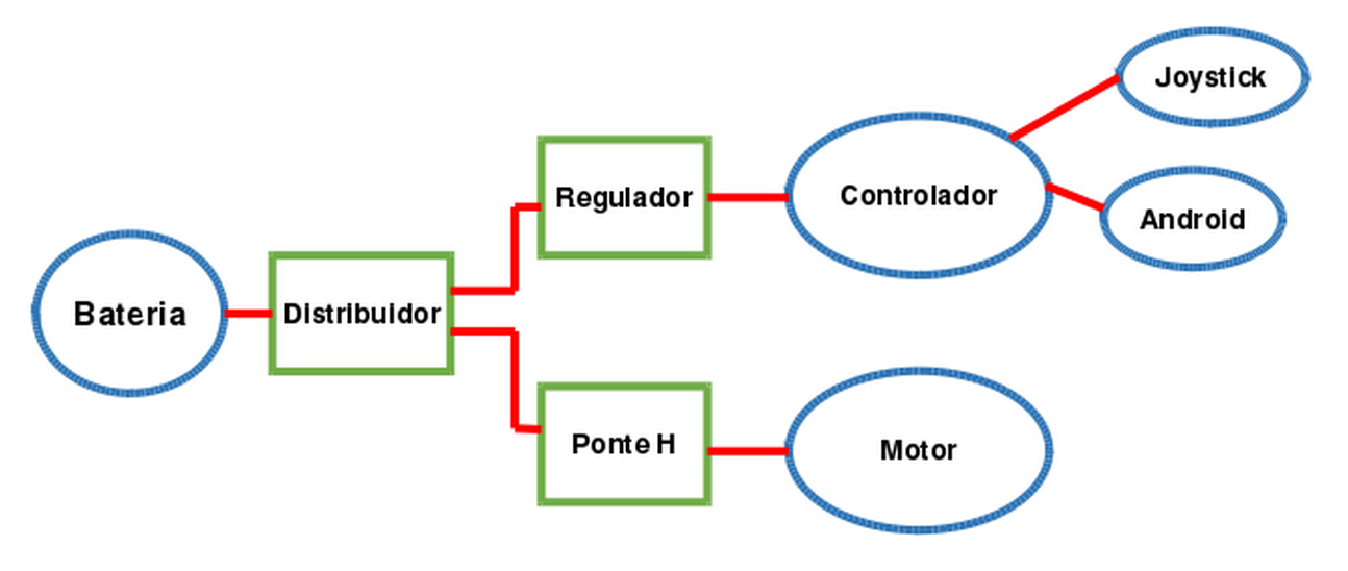
\includegraphics[keepaspectratio=true,scale=0.6]{figuras/controle/esquema_controle}
\caption{Esquemático de funcionamento geral da cadeira de rodas automatizada}
\label{fig:esquema_controle}
\end{figure}


Para o kit de automação da cadeira de rodas, será utilizada a ponte H para o controle dos motores. Um algoritmo de controle PWM usando o Raspeberry Pi que deve responder aos comandos do usuário como direção, aceleração, frenagem, entre outros que serão posteriormente levantados. Na figura \ref{fig:diagrama_blocos} pode ser obervado o esquemático geral do sistema. Tem-se ainda o Distribuidor, uma placa para facilitar a alimentação do sistema, e o Regulador, para alimentar o Controlador e periféricos.

\begin{figure}[!htb]
\centering
  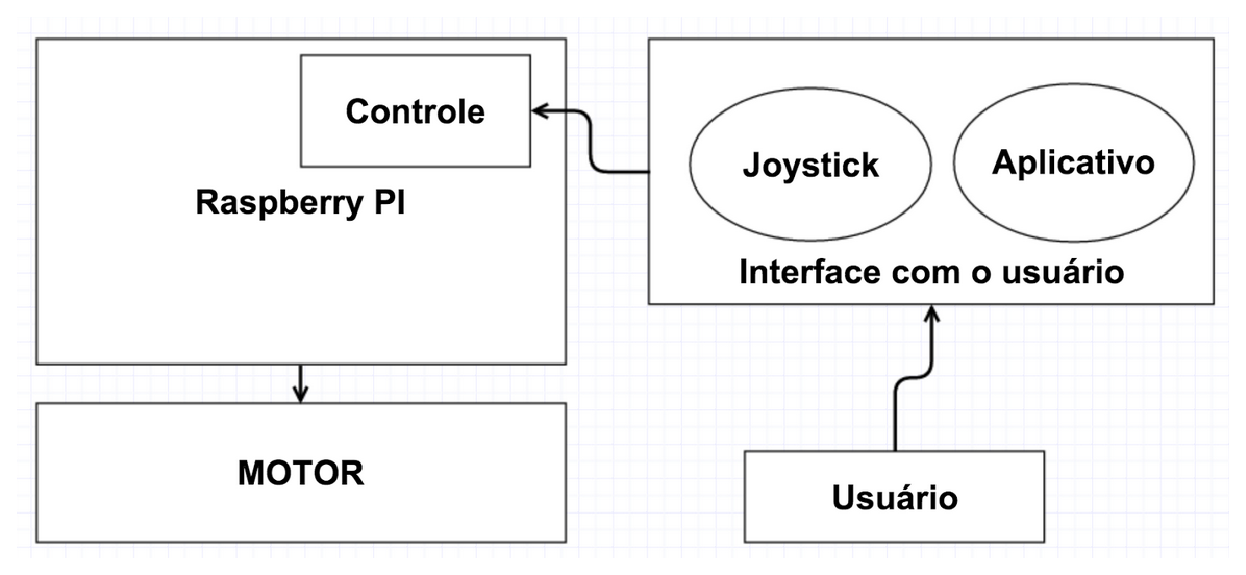
\includegraphics[keepaspectratio=true,scale=0.6]{figuras/controle/diagrama_blocos}
\caption{Desenho do diagrama de blocos do sistema de controle}
\label{fig:diagrama_blocos}
\end{figure}

O sistema vai ser projetado de forma que não seja necessário retirar a bateria para essa ser carregada, o grupo ainda não estabeleceu se o carregador vai ser construído ou comprado, considerando que o tempo disponível para o desenvolvimento do projeto é relativamente curto.

O Distribuidor vai ser basicamente uma placa que facilitara a conexão de todas as outras ao sistema, assim não será necessário que haja reduções de tensão tão drásticas. A placa terá um circuito de proteção, para evitar problemas de sobretensão e curto, saídas para a ponte H, tanto para alimentar possíveis circuitos e motor e ainda saídas para o regulador.

O Regulador terá a funcionalidade de alimentar o controlador com seus periféricos. Essa placa terá um circuito de proteção, para o controlador, contra possíveis problemas do distribuidor, saídas de alimentação para o controlador e ainda uma USB de alimentação para o celular do usuário, para impedir problemas de falta de bateria.

A ponte H será o circuito responsável por fazer o controle de velocidade e direção dos motores. Essa placa terá além dos circuitos necessários para o funcionamento da ponte H, um circuito de proteção para os motores e pinos de entrada do PWM, já que pode haver possíveis problemas de sobretensão a alimentação do motor.


\section{Interface com o usuário}


\subsection{Joystick}
Para as cadeiras de rodas automatizadas essa é uma solução comum de controle para as mesmas, tendo em vista que é relativamente simples de ser acoplado uma vez que se entenda seu funcionamento básico. Para o projeto em questão essa foi uma das alternativas encontradas. No qual o joystick seria acoplado ao braço da cadeira, ou em uma posição que o usuário se sinta mais ergonomicamente confortável. Este acoplamento deve ser simples para favorecer a característica de portabilidade do projeto como um todo.

Caso necessário a conexão do joystick ao sistema de controle pode ser feita por bluetooth, tal característica contribui para o objetivo final do projeto \cite{artigo_joystick_controller}.

\subsubsection{Smartphone}
O \textit{smartphone} é um telefone celular com um sistema operacional móvel avançado que combina as características de um sistema operacional de computador pessoal com outros recursos úteis para uso móvel ou portátil \cite{article_smartphone}.

Devido a portabilidade destes dispositivos e sua facilidade de integração com outros sistemas, uma possível solução para a interação do usuário com o sistema pode ser feita. Uma conexão entre o dispositivo e o sistema será feita através de Bluetooth (Android) ou "Virtual Private Network" (iOS e Android). Para o projeto em questão o usuário pode optar por utilizar o \textit{Smartphone} ou ainda o joystick.

\subsubsection{Protótipo}

O protótipo na figura \ref{fig:prototipos} foi feito com o intuito de mostrar o fluxo do aplicativo sugerido para o controle da cadeira de rodas automatizada.

A principal funcionalidade deste aplicação é basicamente voltada para o controle da cadeira de rodas automatizada, no qual o usuário teria um \textit{joystick} virtual que se comunica com o \textit{Raspeberry Pi} enviando o comando para os motores.
Uma das restrições pensadas, foi a de enquanto o controle estiver ativado via aplicativo o usuário não poderia ter o controle através do \textit{joystick} físico.


  \begin{figure}[!htb]
		\centering
		\legend{}
    \subfloat{
  		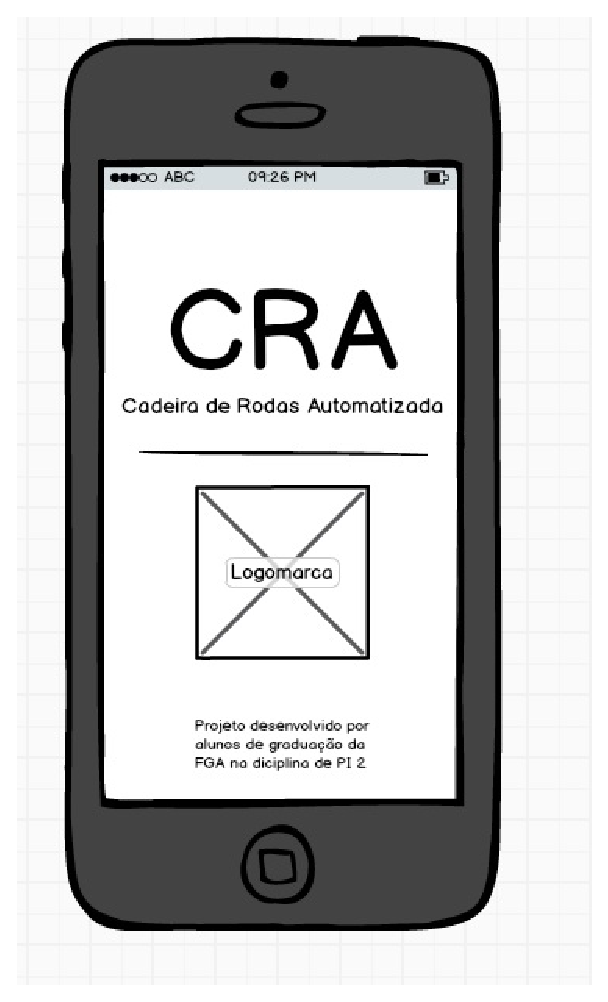
\includegraphics[keepaspectratio=true,scale=0.6]{figuras/controle/tela_1}
		}
		\quad %espaco separador
		\subfloat{
  		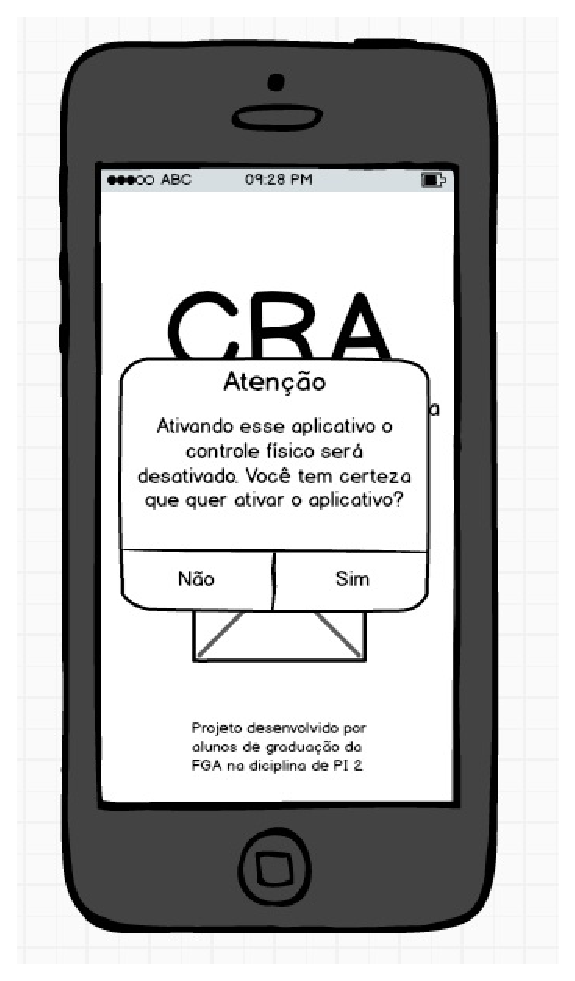
\includegraphics[keepaspectratio=true,scale=0.6]{figuras/controle/tela_2}
		}
		\subfloat{
  		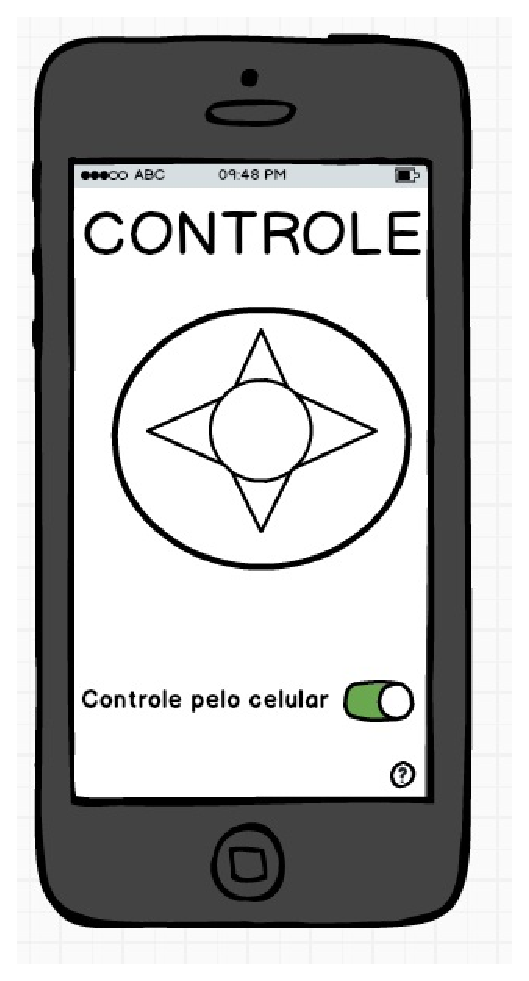
\includegraphics[keepaspectratio=true,scale=0.6]{figuras/controle/tela_3}
		}
		\quad %espaco separador
		\subfloat{
  		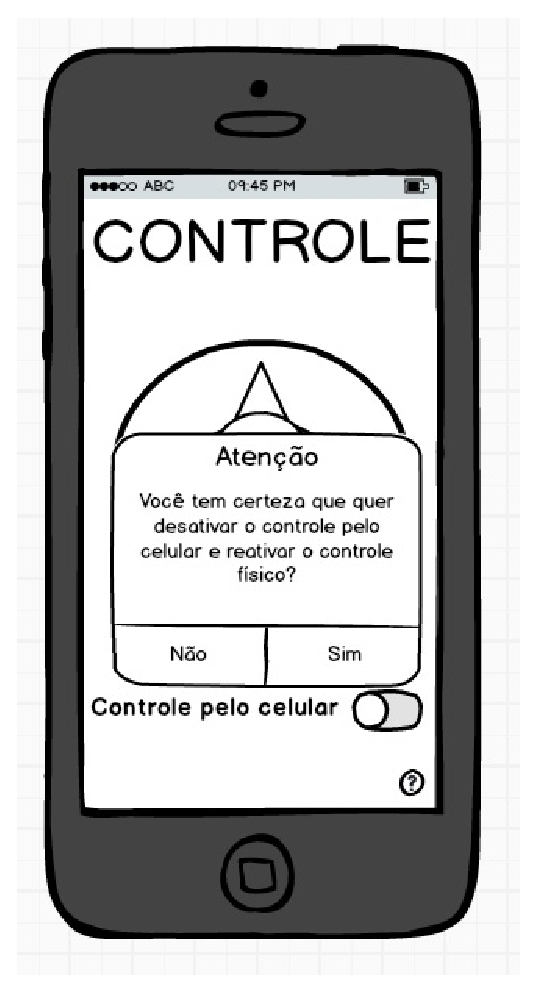
\includegraphics[keepaspectratio=true,scale=0.6]{figuras/controle/tela_4}
		}
		\caption{Protótipo de aplicativo para interface entre usuário e motor}
		\label{fig:prototipos}
  \end{figure}
